\subsubsection{Inciso a}
Sabemos que:
\begin{itemize}
	\item Rojo es flanders
	\item Azul es homero
	\item $b \in \mathbb{R}_{>0}$ es el beneficio de tener taladro
	\item $c \in \mathbb{R}_{>0}$ es el costo de comprar el taladro
	\item $b > c$ $ \implies $ $ b - c > 0$  
\end{itemize}

\begin{definition}	
Sea $G=(V, E)$ un grafo. 
\begin{itemize}
	\item Sea la funcion $f:V \rightarrow \{v \in V\}$ la funcion que dado un nodo $v \in V$ me devuelve los vecinos.
	\item Sea la funcion $g:V \rightarrow \{Homero, Flanders\}$ que dado un nodo me devuelve la estrategia elegida por el. 
	\item Sea la funcion $h: V \rightarrow \mathbb{R}_{\geq 0}$ que dado un nodo me devuelve la utilidad, definida para las siguientes estrategias como:
	\begin{itemize}
		\item \textbf{Ned flanders:} Jugador v, compra el taladro, su utilidad es $h(v) = b-c > 0$  
		\item \textbf{Homero:} Jugador v, no compra el taladro, y se lo pide a un vecino, su utilidad es
		\begin{itemize}
			\item $h(v) = c$  Si $(\exists w \in f(v)/ g(w) = flanders)$. \texttt{Si tiene algun vecino flanders.}
			\item $h(v) = 0$  \texttt{En caso contrario.}
		\end{itemize}	 
	\end{itemize}
\end{itemize}
\end{definition}

\begin{theorem}
	\label{ida-caracterizacion-nash}
	Un grafo que cumple las siguientes condiciones, corresponde a un equilibrio de nash.
	\begin{itemize}
		\item \textbf{Todos los jugadores flanders tienen todos vecinos homero}. $(\forall v \in V / g(v) = flanders) \implies (\forall w \in f(v), g(w) = homero)$ 

		\item \textbf{Todos los jugadores homero tienen al menos un vecino flanders}. $(\forall v \in V / g(v) = homero) \implies (\exists w \in f(v)/ g(w) = flanders)$ 
	\end{itemize}
\end{theorem}

\begin{proof}
Veamos porque un grafo que cumple estas condiciones representa un equilibrio de nash:
\begin{itemize}
	\item A los jugadores v, que juegan homero, con utilidad $h(v) = b > 0$, no les conviene cambiar a flanders porque de hacerlo, tendrian utilidad $h(v) = b - c < b$. \textbf{Les va mejor pidiendo prestado a su vecino flanders.}
	\item A los jugadores v, que juegan flanders, con utilidad $h(v) = b-c > 0$, no les conviene cambiar a homero porque de hacerlo, tendrian utilidad $h(v) = 0 < b - c$, \textbf{ya que no tienen ningun vecino a quien pedirle el taladro.}
\end{itemize}
\end{proof}

\begin{theorem}
	El grafo de la figura es un equilibrio de nash. 
\end{theorem}
\begin{proof}
Asumiendo que el grafo se extiende fuera del grafico de la misma forma. Lo que se observa es que dicho grafo cumple las condiciones mencionadas en \ref{ida-caracterizacion-nash}.
\end{proof}

\subsubsection{Incisos b y c}

\begin{theorem}
	\label{vuelta-caracterizacion-nash}
	Si un grafo G=(V, E) se corresponde a un equilibrio de nash, entonces valen las condiciones enunciadas en \ref{ida-caracterizacion-nash}.
\end{theorem}
\begin{proof}
	Supongamos que no, es decir que alguna de las siguientes es cierta y sigue siendo un equilibrio:\\
	\begin{enumerate}
		\item \textbf{Existe un jugador flanders que tiene otro vecino flanders}. $(\exists v \in V / g(v) = flanders) \implies (\exists w \in f(v), g(w) = flanders)$ 

		\item \textbf{Existe un jugador homero que tiene todos vecinos homero}. $(\exists v \in V / g(v) = homero) \implies (\forall w \in f(v)/ g(w) = homero)$ 
	\end{enumerate}
	En el primer caso, sea v dicho jugador, le conviene cambiar a homero y mejorar su utilidad de $b-c$ a $b > b-c$. Por lo tanto no es un equilibrio. En el segundo caso, sea dicho jugador w, le conviene cambiar a flanders y mejorar su utilidad de 0 a $b-c >0$. Por lo tanto, tampoco es un equilibrio.
\end{proof}

\begin{corollary}
	\label{sii-nash-caracterizacion}
	Usando \ref{ida-caracterizacion-nash} y \ref{vuelta-caracterizacion-nash}. Podemos decir que un grafo representa un equilibrio de nash $\leftrightarrow$ cumple con las condiciones enunciadas en \ref{ida-caracterizacion-nash}.
\end{corollary}

\begin{definition}
	Dado G=(V, E) un grafo, se define $T \subseteq V$ un conjunto independiente de nodos si y solo si $\forall w,v \in T w \neq v$ la arista $(v, w) \notin E$. Es decir, los nodos de T no tienen links entre ellos.
\end{definition}

\begin{definition}
	Un conjunto independiente maximal T, es aquel conjunto independiente tal que no esta contenido en ningun otro conjunto independiente.
\end{definition}

\begin{definition}
	Dado G=(V, E) un grafo, se define $T \subseteq V$ un conjunto dominante de nodos si $\forall v \in (V \setminus T) $ $\exists w \in T $ tal que $ (v, w) \in E$. En castellano, que todo nodo de $(V \setminus T) $ sea vecino de un elemento de $T$.
\end{definition}

\begin{theorem}
	\label{caracterizacion-conjindepdominante}
	Dado G=(V, E) un grafo que representa un equilibrio de nash, $V = F \cup H$ donde F es el conjunto de los nodos que juegan Flanders y H es el conjunto de nodos que juegan Homero. Usando la caracterizacion de \ref{sii-nash-caracterizacion} y las definiciones anteriores. Notemos que F es un conjunto independiente y dominante. Y podemos definir una particion del conjunto de nodos como $V = F \cup (V \setminus F)$ tal que G sigue representando un equilibrio de nash.
\end{theorem}
\begin{proof}
	Veamos que esta particion del conjunto de nodos $V = S \cup (V \setminus S)$ cumple las 2 condiciones enunciadas en \ref{ida-caracterizacion-nash}.
	\begin{enumerate}
		\item $\forall v \in S $ $(\forall w \in f(v), g(w) = homero) $. De lo contrario habria 2 nodos en $S$ con una arista, absurdo porque $S$ es independiente.
		\item Sea $H = (V \setminus S)$, entonces $(\forall v \in H) \implies (\exists w \in f(v)/ g(w) = flanders)$. De lo contrario habria un nodo en $V = (V \setminus S)$ que no es vecino de un nodo en $V$, absurdo porque $S$ es dominante.
	\end{enumerate}
\end{proof}

\begin{theorem}
	Un conjunto independiente maximal V, es tambien un conjunto dominante.
\end{theorem}
\begin{proof}
	Supongamos que no, luego tenemos un elemento $w \in (V \setminus S)$ tal que $(w, v) \notin E$ para ningun $v \in V$, entonces si considero $T = V \cup \{w\}$ tambien es un conjunto independiente, lo cual es absurdo, porque V era maximal.
\end{proof}

\begin{theorem}
	\label{nash-cjind}
	Dado G=(V, E) un grafo, un algoritmo que me construya un conjunto independiente maximal S, me genera una particion de nodos $V = S \cup (V \setminus S)$ tal que si tomo $V$ como los nodos que juegan flanders y $(V\setminus S)$ como los nodos que juegan homero, tengo un equilibrio de nash. En definitiva, tal algoritmo me genera equilibrios de nash sobre el grafo G.
\end{theorem}
\begin{proof}
	Sale del teorema \ref{caracterizacion-conjindepdominante}.
\end{proof}

\begin{theorem}
	\label{Multiplicidad-cjindmax}
	Sea G = (V, E) un grafo con al menos una arista tiene mas de un conjunto maximal independiente.
\end{theorem}
\begin{proof}
	Consideremos la arista $(v, w)\in E$ que menciona la hipotesis. Ahora consideremos $C_1$ y $C_2$ conjuntos independientes maximales, construidos golosamente a partir de v y w. Debe valer $C_1 \neq C_2$ pues de lo contrario los nodos v, w de la arista estarian en el mismo conjunto independiente, lo cual es absurdo, porque el conjunto es independiente. Luego encontramos mas de un conjunto maximal independiente,como queriamos ver.  

\end{proof}
\begin{theorem}[Existencia de multiples equilibrios de nash]
	Sea G=(V, E) un grafo finito con mas de dos jugadores conectados. Luego existe un equilibrio de nash, y no es unico.
\end{theorem}
\begin{proof}
	Usando los teoremas \ref{nash-cjind} y \ref{Multiplicidad-cjindmax}. Aplicando el algoritmo sobre nodos iniciales v,w tales que $(v,w) \in E$, para que el conjunto independiente computado sea distinto.
\end{proof}

\begin{theorem}[Algoritmo goloso de busqueda de un conjunto maximal]
	Sea G = (V, E), donde V es el conjunto de nodos del grafo, entonces:
	\begin{enumerate}
		\item Sea $I = \emptyset$
		\item Mientras haya nodos en V repetir
		\begin{itemize}
			\item Elegir un nodo $v_i$ de el conjunto $V$
			\item $I = I \cup \{v\} $
			\item $V = V \setminus (\{v\} \cup f(v)) $, donde f(v) son los vecinos del nodo v.
		\end{itemize}
		\item Devolver I.
	\end{enumerate}
	I es un conjunto independiente maximal de G.
\end{theorem}

\subsubsection{Inciso d}

Se pide hallar familias de grafos de n nodos, conexos, tales que:
\begin{enumerate}
	\item \textbf{Una familia de grafos tal que el numero de taladros sea independiente de n.} Vemos que en la familia de nodos $K_n$, o grafos completos, grafos donde estan presentes las aristas entre cada par de nodos, el numero de taladros necesarios para un equilibrio de nash es independiente de n. Mas aun, con un jugador que juegue flanders, y n-1 que jueguen homero. Se cumplen ambas propiedades mencionadas en \ref{ida-caracterizacion-nash}, con las cuales justificamos en el inciso a que es un equilibrio de nash.
	\begin{figure}[H]
	  \centering	
		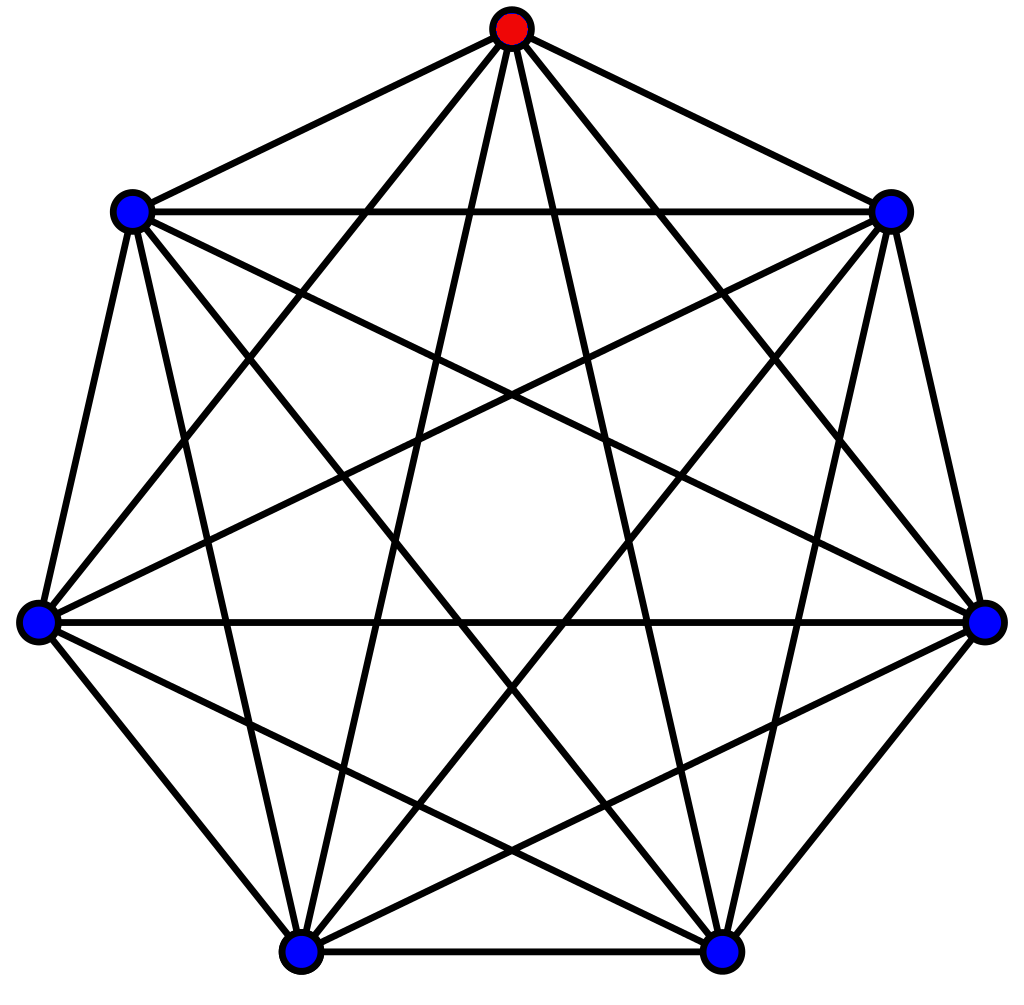
\includegraphics[scale=0.20]{fig/Kn.png}
	  \caption{Grafo del item 3.d.1}
	\end{figure}

	\item \textbf{Una familia de grafos tal que el equilibrio de nash necesita al menos $\frac{n}{2}$ taladros, pero existe una distribucion de taladros tal que 2 sean suficientes para que todos tengan un taladro o tengan un vecino que tenga taladro.} Vemos que para este caso podemos considerar la familia de grafos indicada en las figuras debajo. \ref{3d2} y \ref{3d2b}.
	\begin{figure}[H]
		\label{3d2}
	  \centering	
		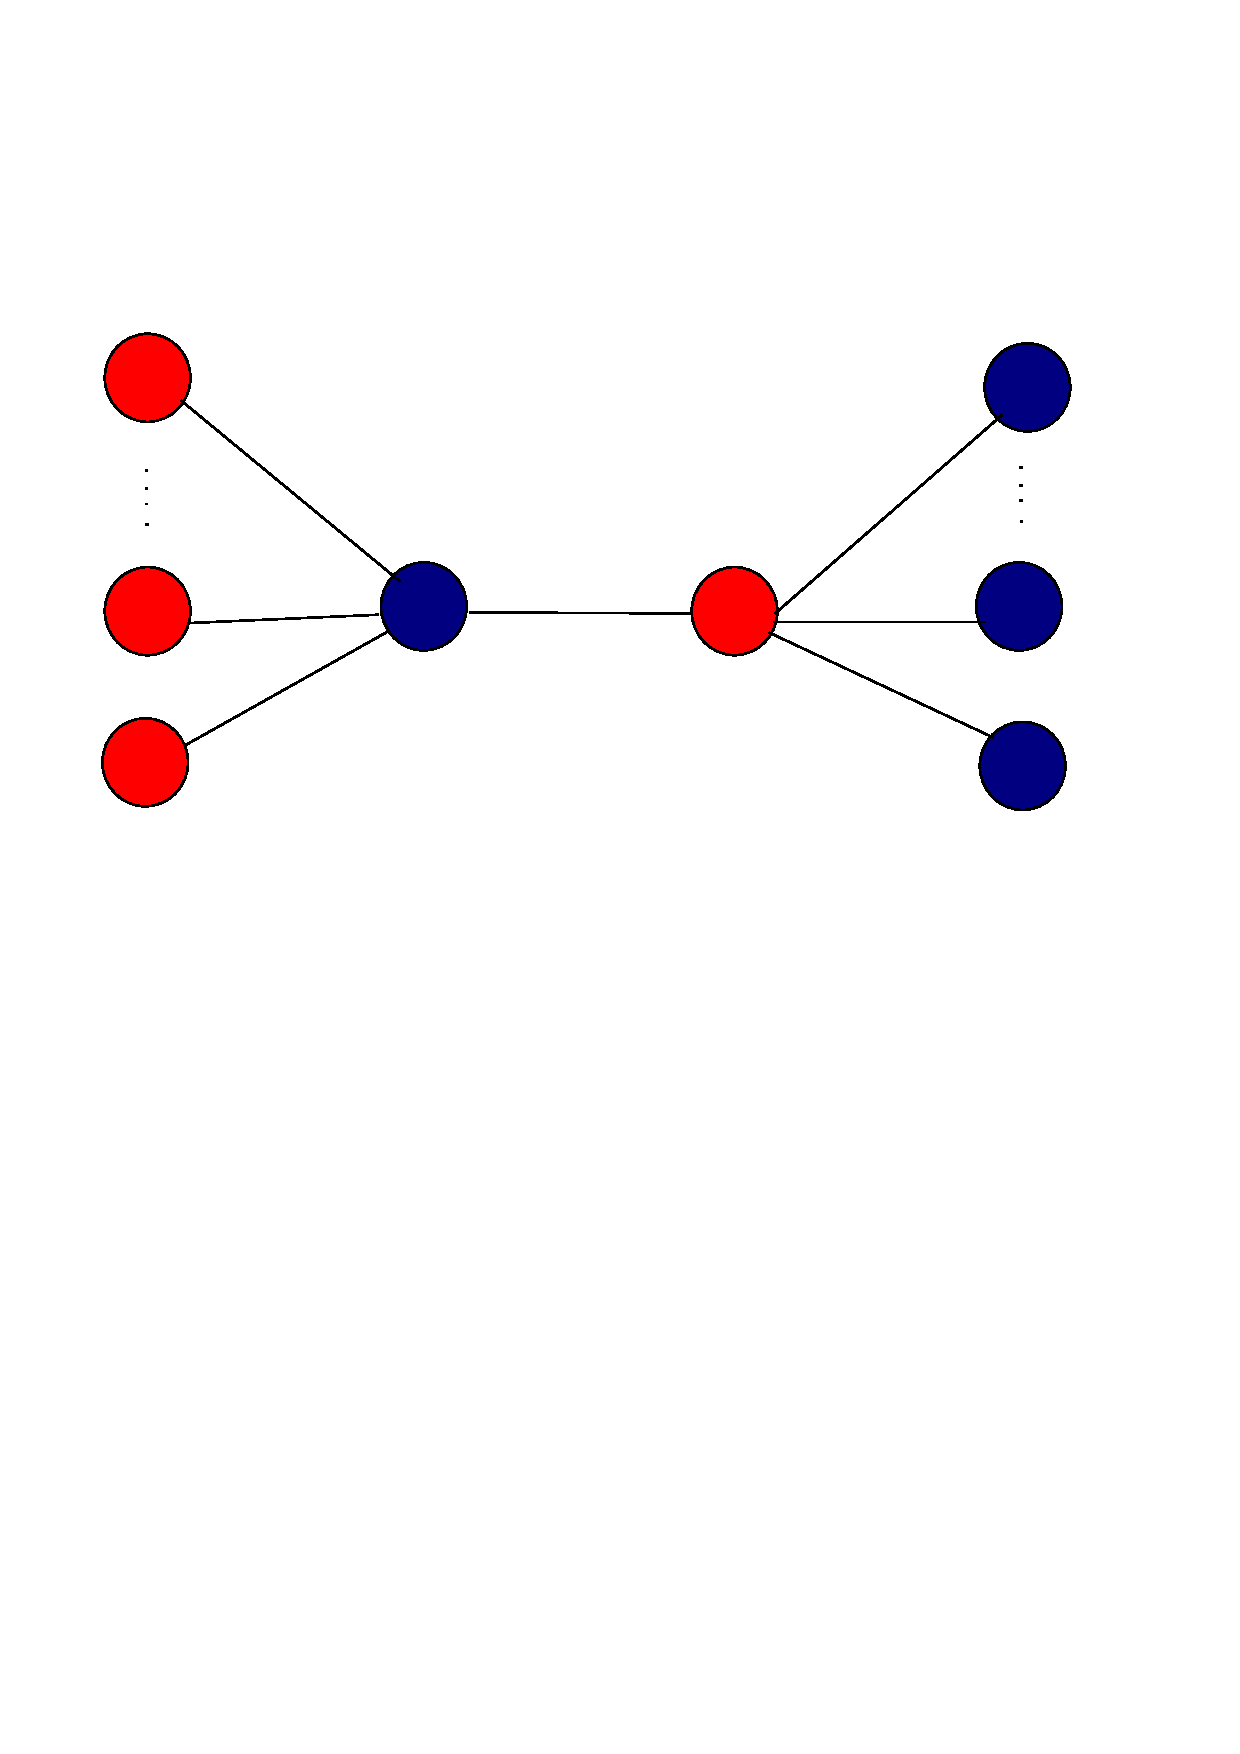
\includegraphics[scale=0.30]{fig/grafo3d2.pdf}
	  \caption{Grafo del item 3.d.2 exhibiendo la condicion de n/2 taladros.}
	\end{figure}

	\begin{figure}[H]
		\label{3d2b}
	  \centering	
		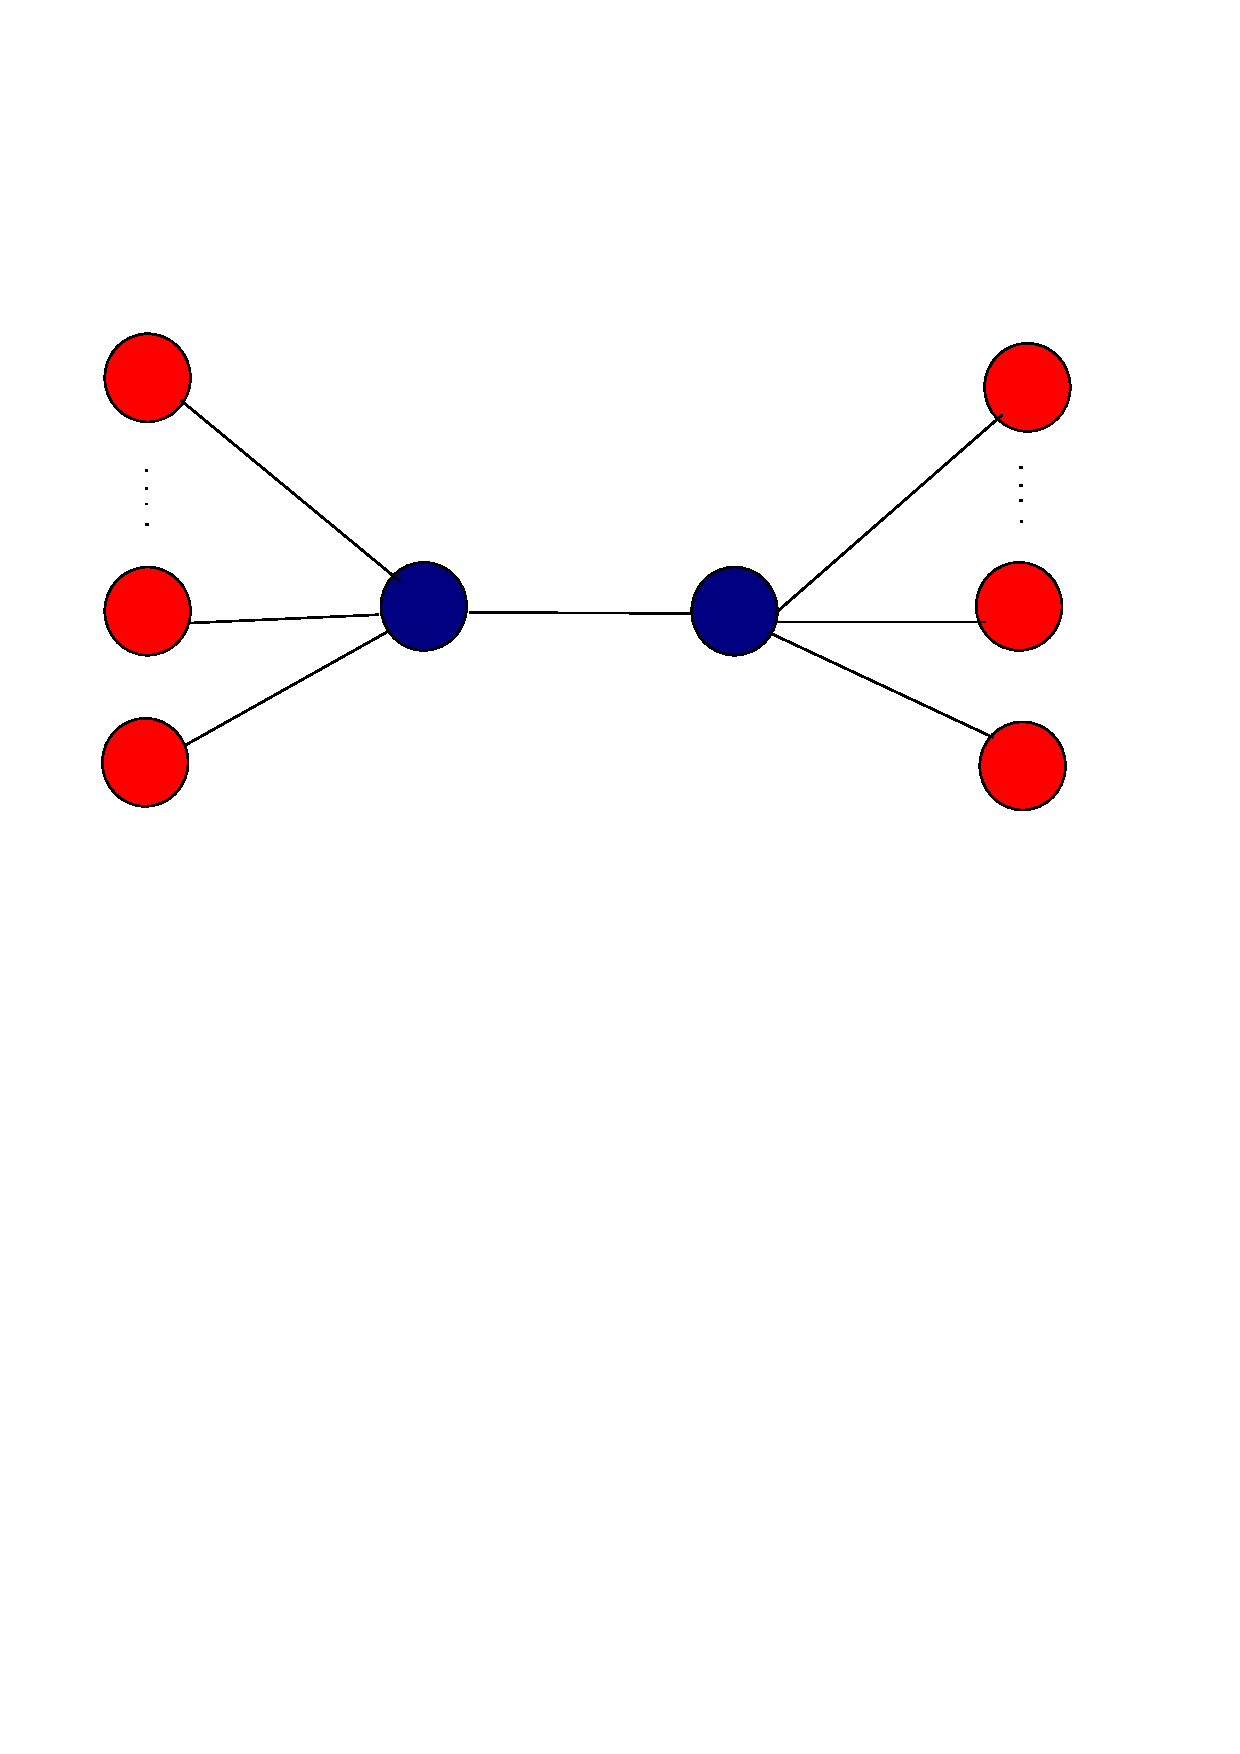
\includegraphics[scale=0.30]{fig/grafo3d2b.pdf}
	  \caption{Grafo del item 3.d.2 exhibiendo la condicion de 2 taladros}
	\end{figure}

	\item \textbf{Una familia de grafos tal que todo equilibrio de nash usa aproximadamente una fraccion $\frac{n}k{}, k \in \mathbb{N}$, asumimos que si el grafo es conexo, no es union de grafos disjuntos.(pues hay una arista que los une, entonces no son disjuntos)}. Vemos que es casi una generalizacion del item anterior. Notemos que la fraccion $\frac{n}{k}$ es \textbf{aproximada}. \\
	La idea es tener \texttt{nubes} de $\frac{n}{k}$ nodos sin conexion, cada nube se corresponderia con un grafo ${K_{\frac{n}{k}}}^c$. Luego una arista central, con dos nodos, llamemoslos $v_1$ y $v_2$. El conjunto de aristas del grafo quedaria determinado por las siguientes reglas:
	\begin{enumerate}
		\item $v_1$ y $v_2$ son vecinos.
		\item Para toda nube $n_i$, $i \in\{1,...k-2\}$ , todos sus nodos $n_{i,j}$, estan conectados con $v_1$ y $v_2$ por las aristas $(n_{i,j}, v_1) \in E$ y $(n_{i,j}, v_2) \in E$

		\item La nube $n_{k-1}$ tiene todos sus nodos conectados a $v_1$ por las aristas $(n_{k-1,j}, v_2) \in E$
		\item La nube $n_{k}$ tiene todos sus nodos conectados a $v_2$ por las aristas $(n_{k,j}, v_2) \in E$
	\end{enumerate}
	Las reglas de disposicion de estrategias es como sigue a continuacion:
	\begin{enumerate}
		\item Para toda nube $n_i$, $i \in\{1,...k-1\}$ todos sus nodos juegan homero.
		\item El nodo central $v_1$ juega flanders.
		\item El nodo central $v_2$ juega homero.
		\item La nube $n_k$, tiene todos sus nodos jugando flanders.
	\end{enumerate}
	Puede pensarse una asignacion simetrica cambiando las estrategias de v1 y v2, y las ultimas 2 nubes en la enumeracion.\\
	Es facil ver, dadas estas reglas, que valen las condiciones de \ref{sii-nash-caracterizacion},por lo tanto es un equilibrio de nash. Ademas, veamos que hay asignados $1 + \frac{n}{k}$ taladros.
%	\begin{figure}[H]
%		\label{3d2b}
%	  \centering	
%		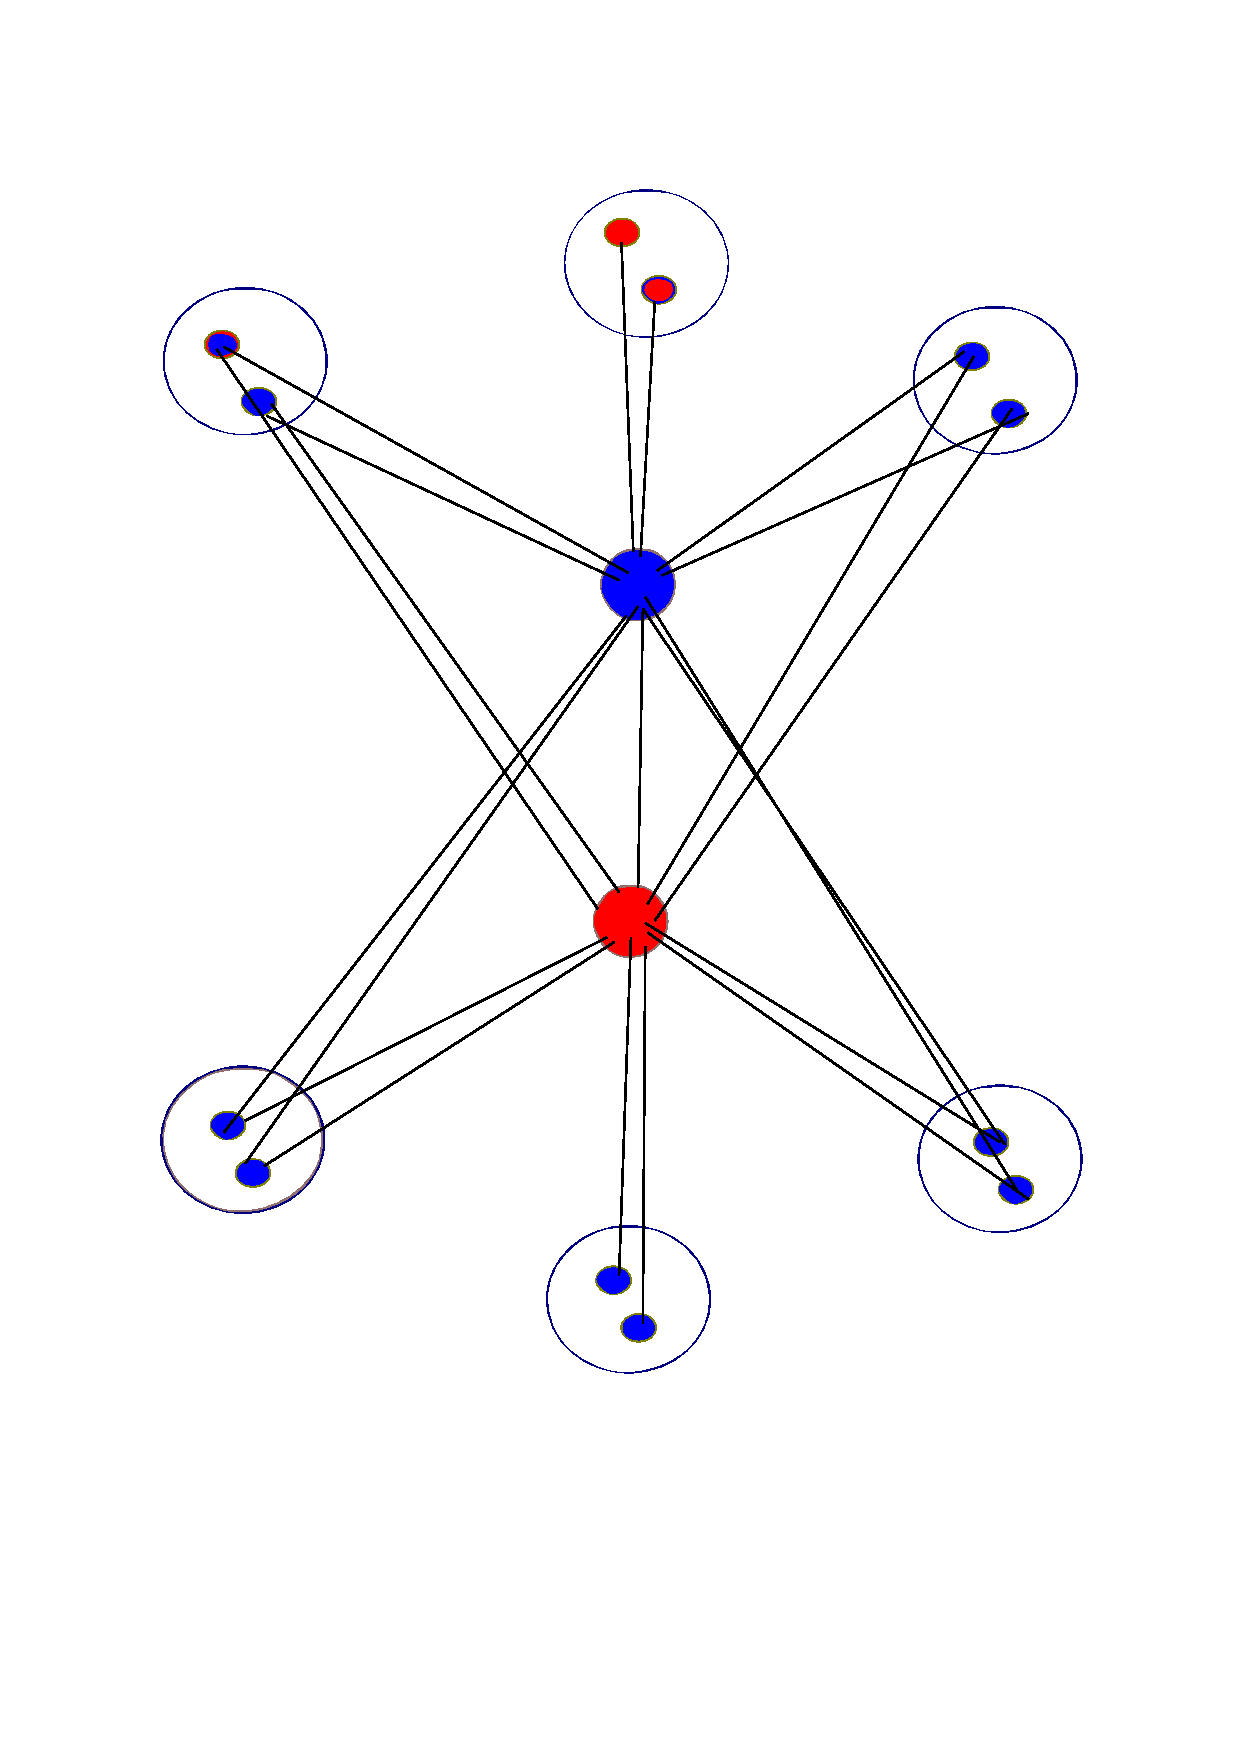
\includegraphics[scale=0.30]{fig/grafo3d3.pdf}
%	  \caption{Grafo del item 3.d.3}
%	\end{figure}
\end{enumerate}

